\documentclass[a4paper,11pt]{article}
% Various packages
\usepackage{siunitx}
\usepackage[utf8]{inputenc} % æøå
\usepackage[T1]{fontenc} % mere æøå
\usepackage[danish]{babel} % orddeling
\usepackage{verbatim} % så man kan skrive ren tekst
\usepackage{graphicx}
\graphicspath{{assets/}}
\usepackage{a4wide}
\usepackage{url}
\usepackage[left=2cm,top=2cm,bottom=1.5cm,right=2cm]{geometry}
\usepackage{amsmath}
\usepackage{amssymb}
\usepackage{amsthm}
\usepackage{wrapfig}
\usepackage{fixme}
\usepackage{color}
\usepackage{pstricks}
\usepackage{pdfpages} % include pdf
\usepackage{float} % Use [H] in figures
\usepackage{subcaption} % For subfigures
\usepackage{color} % May be necessary if you want to color links
\usepackage{hyperref} % Make references clickable
\usepackage[nameinlink,capitalize]{cleveref} % Make eq:refs be in style (1)
\usepackage[linesnumbered, commentsnumbered, lined, ruled, vlined,
%noend  % Have no ⌊-like symbol to indicate end of scope in pseudocode
]{algorithm2e} % Doc: https://goo.gl/6bC1qZ

% Ændr på navnene der vises når man bruger \autoref{label}
\def\sectionautorefname{Sektion}
\renewcommand{\equationautorefname}{Ligning}
\def\figureautorefname{Figur}
\AtBeginDocument{\renewcommand{\ref}[1]{\autoref{#1}}}

% Sæt \ref{} til at kalde \autoref{}
\AtBeginDocument{\renewcommand{\ref}[1]{\autoref{#1}}}

% Ændr ''*'' i math-felter til \cdot
\DeclareMathSymbol{*}{\mathbin}{symbols}{"01}

% Sæt farver for interne referencer og links
\definecolor{darkblue}{RGB}{25,25,112}
\hypersetup{
	colorlinks=true,    %set true if you want colored links
	linktoc=all,        %set to all if you want both sections and subsections linked
	linkcolor=darkblue, %choose some color if you want links to stand out
	filecolor=blue,     %
	citecolor=black,    %
	urlcolor=cyan,      %
}

% Set indentation to 0:
\setlength\parindent{0pt}

% Keywords relateret til algorithm2e pakken
\newcommand{\True}{\textbf{true}}\newcommand{\False}{\textbf{false}}
\SetStartEndCondition{ }{}{}%
\SetKwProg{Fn}{def}{\string:}{}
\SetKw{KwTo}{to}
\SetKwFor{For}{for}{}{}% 
\SetKwFor{ForEach}{foreach}{}{}% 
\SetKwIF{If}{ElseIf}{Else}{if}{}{elif}{else}{end}% 
\SetKwFor{While}{while}{}{end}\SetKwProg{Fn}{}{}{}
\SetKwInOut{Input}{input}\SetKwInOut{Output}{output}
\setlength{\algomargin}{3em}\DontPrintSemicolon

\newcommand{\longspace}{{\ \ \ \ \ \ \ \ \ \ \ \ \ \ }}
\renewcommand{\P}{{\mathbb P}}
\newcommand{\parfrac}[1]{\frac{\partial}{\partial #1}}
\renewcommand{\num}{{\textrm{num} }}
\newcommand{\size}{{\textrm{size} }}
\newcommand{\ift}{{\textrm{if } }}

% Dynamiske (), <>, ceil, floor
\newcommand{\p}[1]{\left( #1 \right)}
\newcommand{\pbig}[1]{\big( #1 \big)}
\newcommand{\pBig}[1]{\Big( #1 \Big)}
\newcommand{\pbigg}[1]{\bigg( #1 \bigg)}
\newcommand{\larr}[1]{\left< #1 \right>}
\newcommand{\ceil}[1]{\left\lceil #1 \right\rceil}
\newcommand{\floor}[1]{\left\lfloor #1 \right\rfloor}


% Squiggly arrows
\DeclareFontFamily{U} {MnSymbolC}{}

\DeclareFontShape{U}{MnSymbolC}{m}{n}{
	<-6> MnSymbolC5
	<6-7> MnSymbolC6
	<7-8> MnSymbolC7
	<8-9> MnSymbolC8
	<9-10> MnSymbolC9
	<10-12> MnSymbolC10
	<12-> MnSymbolC12}{}
\DeclareFontShape{U}{MnSymbolC}{b}{n}{
	<-6> MnSymbolC-Bold5
	<6-7> MnSymbolC-Bold6
	<7-8> MnSymbolC-Bold7
	<8-9> MnSymbolC-Bold8
	<9-10> MnSymbolC-Bold9
	<10-12> MnSymbolC-Bold10
	<12-> MnSymbolC-Bold12}{}

\DeclareSymbolFont{MnSyC} {U} {MnSymbolC}{m}{n}

\DeclareMathSymbol{\MNrhd}{\mathbin}{MnSyC}{76}
\DeclareMathSymbol{\MNlhd}{\mathbin}{MnSyC}{78}
% =============================================
\DeclareFontFamily{U} {MnSymbolD}{}

\DeclareFontShape{U}{MnSymbolD}{m}{n}{
	<-6> MnSymbolD5
	<6-7> MnSymbolD6
	<7-8> MnSymbolD7
	<8-9> MnSymbolD8
	<9-10> MnSymbolD9
	<10-12> MnSymbolD10
	<12-> MnSymbolD12}{}
\DeclareFontShape{U}{MnSymbolD}{b}{n}{
	<-6> MnSymbolD-Bold5
	<6-7> MnSymbolD-Bold6
	<7-8> MnSymbolD-Bold7
	<8-9> MnSymbolD-Bold8
	<9-10> MnSymbolD-Bold9
	<10-12> MnSymbolD-Bold10
	<12-> MnSymbolD-Bold12}{}

\DeclareSymbolFont{MnSyD} {U} {MnSymbolD}{m}{n}
\DeclareMathSymbol{\MNsim}{\mathbin}{MnSyD}{2}

% =============================================

\usepackage{amssymb,amsmath,stackengine}
\stackMath
\newcommand\rsquigarrow[1]{%
	\mathbin{\stackon[2pt]{\rightsquigarrow}{\scriptscriptstyle #1 }}
}

\author{Søren Mulvad, rbn601}

\title{Eksamensdisposition - Dynamisk programmering}
\begin{document}
\maketitle

% Desuden skal hver studerende i gruppen udarbejde en individuel disposition for emnet "Dynamic Programming", som er et af emnerne til eksamen. En disposition skal bestå af de vigtigste punkter, du vil komme ind på til eksamen.
% Tænk på dispositionen som noget, du kan have med dig til eksamen, og som kan hjælpe dig med at huske, hvad du overordnet vil gennemgå til emnet "Divide and Conquer".
% Dispositionen skal ikke indeholde detaljerede beviser og lignende, men de mere overordnede delemner. Sørg for at gøre den kortfattet - f.eks. 5-10 punkter med stikord/-sætninger.

\begin{itemize}
\item \textbf{Paradigmet}
\item \textbf{Eksempel med beregning af Fibonacci}
\item \textbf{Bevis af Theorem 15.1 (\textit{Optimal delstruktur af en LCS})}
\item \textbf{Håndkørsel af \texttt{LCS}}
\begin{itemize}
	\item $X = ABA$ og $Y = BA$
\end{itemize}

\end{itemize}




%%%%%%%%%%%%%%%%%%%%%%%%%%%%%%%%%%%%%%%%%%%%%%%%%%%%%%%%%%%
%%%%%%%%%%%%%%%%%%%%%%%%%%%%%%%%%%%%%%%%%%%%%%%%%%%%%%%%%%%
%%%%%%%%%%%%%%%%%%%%%%%%%%%%%%%%%%%%%%%%%%%%%%%%%%%%%%%%%%%
\newpage
%%%%%%%%%%%%%%%%%%%%%%%%%%%%%%%%%%%%%%%%%%%%%%%%%%%%%%%%%%%
%%%%%%%%%%%%%%%%%%%%%%%%%%%%%%%%%%%%%%%%%%%%%%%%%%%%%%%%%%%
%%%%%%%%%%%%%%%%%%%%%%%%%%%%%%%%%%%%%%%%%%%%%%%%%%%%%%%%%%%
\section{Dynamisk Programmering}



\begin{itemize}
\item \textbf{Paradigmet}
\begin{itemize}
\item Minder en anelse om del og hersk-paradigmet: Del problemet ind i mindre delproblemer, løs delproblemerne rekursivt og kombiner herefter løsningerne.
\item Forskellen ligger i, at problemerne har \textit{optimal delstruktur}. Det vil sige delproblemerne på en eller anden måde overlapper. Altså når flere delproblemer har de samme deldelproblemer. Det kunne f.eks. være når vi skal beregne et Fibonacci tal eller i det jeg vil vise med LCS.
\end{itemize}

%\item \textbf{Udvikling af dynamisk programmering algoritme}
%\begin{enumerate}
%\item Karakterisér strukturen af en optimal løsning
%\item Definer rekursivt værdierne for en optimal løsning
%\item Beregn værdien for en optimal løsning (i virkelighedens verden typisk med bottom-up tilgangen)
%\item Konstruer en optimal løsning ud fra det beregnede (kan udelades hvis man blot vil have f.eks. summen af bekostningen ved en optimal løsning)
%\end{enumerate}

\item \textbf{Eksempel med Fibonacci}\\
\begin{figure}[H]
	\begin{center}
		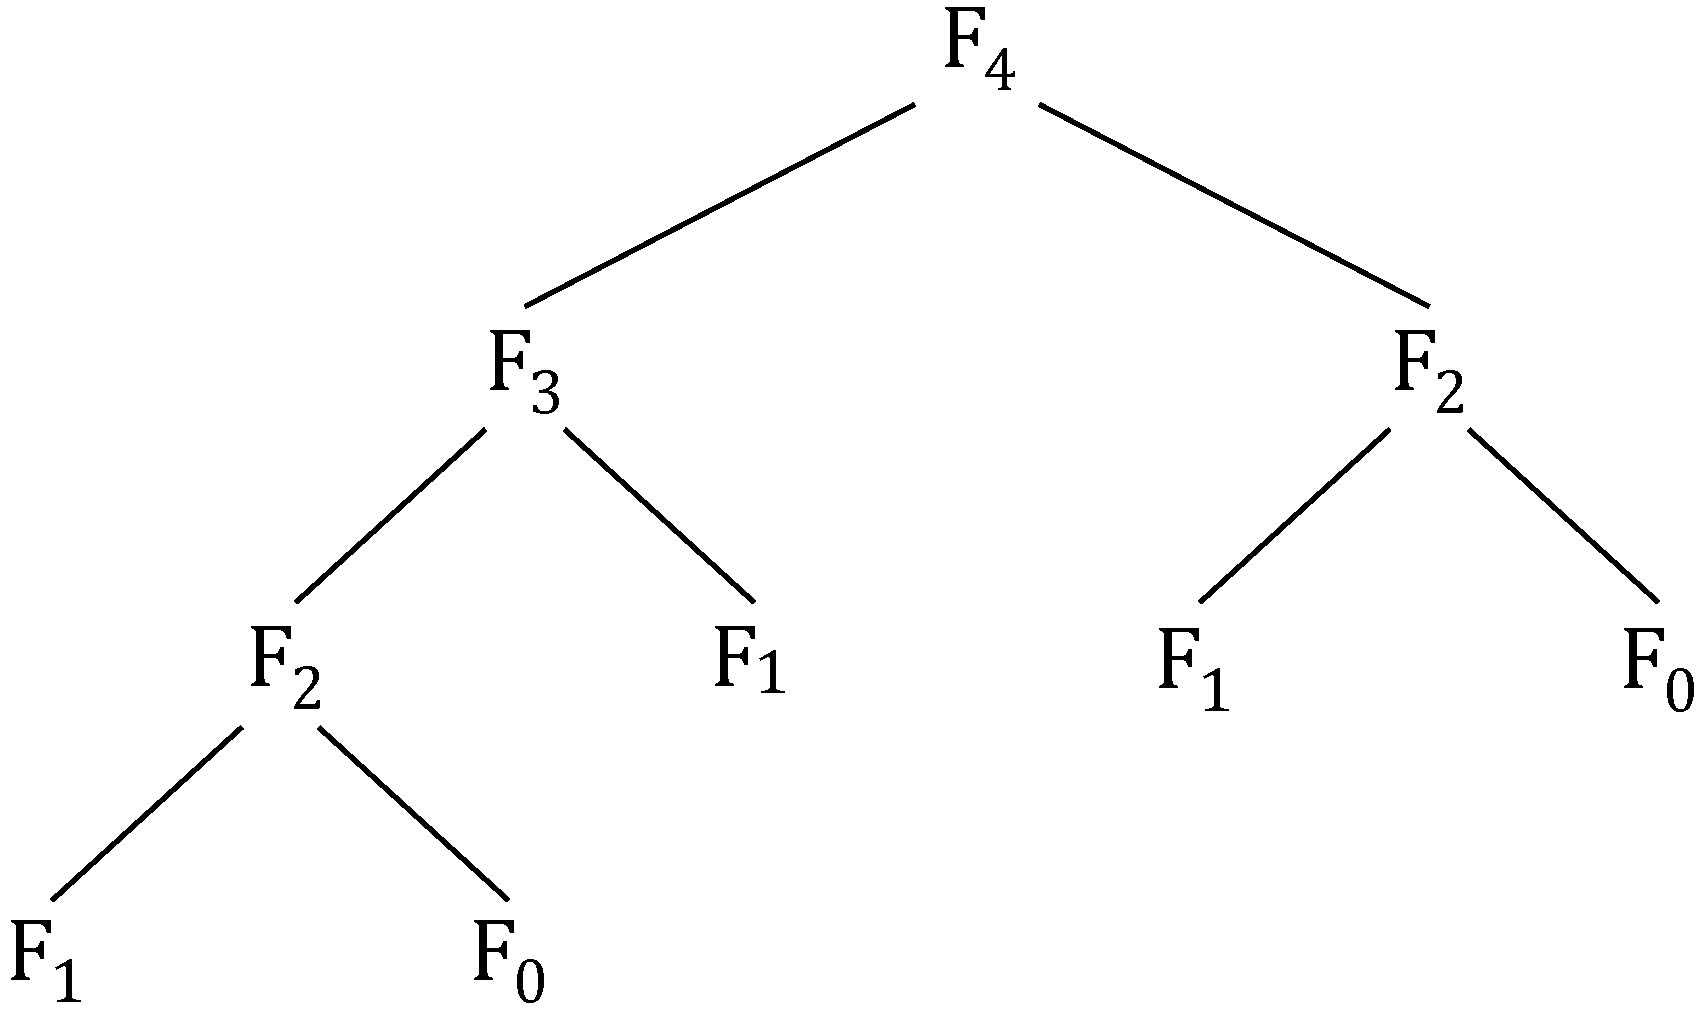
\includegraphics[width=0.5\textwidth]{fib.pdf}
	\end{center}
	\caption{Problemer der skal løses i Fib. Her ser vi, at $F_2$ optræder flere gange.}
	\label{fig:fib}
\end{figure}

Uden DP er køretiden eksponentiel, med DP er køretiden $O(n)$ (såfremt vi kan lægge store tal sammen i konstant tid).


\item \textbf{Beskrivelse af LCS-problemet}\\
Vi vil gerne finde Longest Common Subsequence af f.eks. to DNA-strenge.\\
Hvis vi f.eks. har $S_1 = ACCG$ og $S_2 = AG$ ville den længste den længste sekvens være $AG$, og længden er hermed 2. 

\item \textbf{Theorem 15.1 (\textit{Optimal delstruktur af en LCS})}\\
Lad $X = \left<x_1, x_2, ..., x_m\right>$ og $Y = \left<y_1, y_2, ..., y_n\right>$ være sekvenserne (f.eks. DNA-strenge), og lad $Z = \left<z_1, z_2, ..., z_k\right>$ være en hvilken som helst LCS af $X$ og $Y$:
\begin{enumerate}
	\item[\textbf{1:}] Hvis $x_m = y_n$, så er $z_k = x_m = y_n$ og $Z_{k-1}$ er en LCS af $X_{m-1}$ og $Y_{n-1}$.
	\item[\textbf{2:}] Hvis $x_m \neq y_n$ og $z_k \neq x_m$, så medfører det at $Z$ er en LCS af $X_{m-1}$ og $Y$.
	\item[\textbf{3:}] Hvis $x_m \neq y_n$ og $z_k \neq y_n$, så medfører det at $Z$ er en LCS af $X$ og $Y_{n-1}$.
\end{enumerate}\vspace{1em}


\item \textbf{Beviser af Theorem 15.1}\\
Alle er modstridsbeviser. Tegn strenge ala. følgende for at understøtte argumentation:
\begin{verbatim}
X: *****A
Y: ****A
Z: **A
\end{verbatim}

\begin{enumerate}
	\item[\textbf{1:}]
	Antag $z_k \neq x_m$. Så kunne vi appende $x_m = y_n$ på $Z$, hvorved vi fik en CS af $X$ og $Y$ med en længde $k+1$.\\
	Men vi antog jo netop at $Z$ var en \textit{longest} common subsequence med længden $k$, og derfor har vi en modstrid. Altså er $z_k = x_m = y_n$.\\
	
	Antag $Z_{k-1}$ ikke LCS af $X_{m-1}$ og $Y_{n-1}$. Da $Z_{k-1}$ er CS af $X_{m-1}$ og $Y_{n-1}$, men ikke den længste pr. vores antagelse, så må der findes en anden delstreng $W$ som er CS af $X_{m-1}$ og $Y_{n-1}$, og som er længere hvorved $|W| > |Z_{k-1}| = k-1$.\\
	Men så kunne vi appende $x_m = y_n$ til $W$, og herved få en CS af $X$ og $Y$ med længden $|W| + 1 > k$. Nu har vi fundet en fælles delstreng af $X$ og $Y$, som er længere end vores længste delstreng, hvilket er en modstrid.\\
	
	
	\item[\textbf{2:}]
	Antag $Z$ ikke LCS af $X_{m-1}$ og $Y$. $Z$ er stadig CS fordi vi antager $z_k \neq x_m$. Fordi vi antager det ikke er den længste delstreng, så findes der en delstreng $W$ som er CS af $X_{m-1}$ og $Y$ og længere end $Z$, altså $|W| > |Z|$.\\
	Men $W$ er også CS af $X$ og $Y$, og dermed længere end vores længste delstreng, hvilket er en modstrid.\\
	
	
	\item[\textbf{3:}]
	Symmetrisk med 2.

\end{enumerate}\vspace{1em}


\item \textbf{Håndkørsel af \texttt{LCS}}
\begin{itemize}
	\item 
Ud fra vores Theorem kan vi se, at vi får følgende formel for hvad der skal være på plads $c[i, j]$, idet det angiver længden af en LCS for $X_i$ og $Y_j$:
$$
c[i, j] = \begin{cases}
	0 & \text{hvis $i = 0$ eller $j = 0$}\\
	c[i-1, j-1] + 1 & \text{hvis $i,j > 0$ og $x_i = y_j$}\\
	\max(c[i, j-1], c[i-1, j]) & \text{hvis $i,j > 0$ og $x_i \neq y_j$}
\end{cases}
$$

Vi ser at det er rekursivt defineret, og løsningerne til visse delproblemer vil optræde flere gange. Derfor er det optimalt at løse med dynamisk programmering. Jeg vil nu give en håndkørsel af en implementering der er bottom-up:

\item Eksempel hvor $X = ABA$ og $Y = BA$:
\begin{table}[H]
	\centering
	\begin{tabular}{lllll}
		& $j$ & 0 & 1 & 2 \\
		$i$ &  &  & $B$ & $A$ \\ \cline{3-5} 
		0 & \multicolumn{1}{l|}{} & \multicolumn{1}{l|}{0} & \multicolumn{1}{l|}{0} & \multicolumn{1}{l|}{0} \\ \cline{3-5} 
		1 & \multicolumn{1}{l|}{$A$} & \multicolumn{1}{l|}{0} & \multicolumn{1}{l|}{\begin{tabular}[c]{@{}l@{}}$\uparrow$\\ 0\end{tabular}} & \multicolumn{1}{l|}{\begin{tabular}[c]{@{}l@{}}$\nwarrow$\\ 1\end{tabular}} \\ \cline{3-5} 
		2 & \multicolumn{1}{l|}{$B$} & \multicolumn{1}{l|}{0} & \multicolumn{1}{l|}{\begin{tabular}[c]{@{}l@{}}$\nwarrow$\\ 1\end{tabular}} & \multicolumn{1}{l|}{\begin{tabular}[c]{@{}l@{}}$\uparrow$\\ 1\end{tabular}} \\ \cline{3-5} 
		3 & \multicolumn{1}{l|}{$A$} & \multicolumn{1}{l|}{0} & \multicolumn{1}{l|}{\begin{tabular}[c]{@{}l@{}}$\uparrow$\\ 1\end{tabular}} & \multicolumn{1}{l|}{\begin{tabular}[c]{@{}l@{}}$\nwarrow$\\ 2\end{tabular}} \\ \cline{3-5} 
	\end{tabular}
\end{table}

\item Vi får nu en køretid $O(nm)$ og et umiddelbart pladsforbrug $O(nm)$.\\

Såfremt vi kun er interesserede i hvor lang den længste delstreng er, men ikke hvilke bogstaver den består af, kan vi forbedre pladsforbruget til $O\pBig{\min(n, m)}$. Det gøres ved at vælge den mindste delstreng til at være i toppen, og kun gemme den nuværende række samt rækken lige over.

\item Fordelene ved bottom-up, som vi bruger her, er at vi undgår rekursion og derfor ofte vil have lavere konstantled i forhold til top-down. Fordelen ved top-down er tilgengæld, at vi kun beregner de delproblemer som der faktisk er behov for, for at løse det oprindelige problem hvorimod bottom-up regner alle.


\end{itemize}


\item \textbf{Bonusviden om \texttt{Cut-Rod} til eventuelle spørgsmål}
\begin{enumerate}
	\item Der er et optimalt indeks $i$ hvor vi kan cutte stangen op i to mindre delstange (delproblemer) - denne kan være evt. være $0$:
	$$
	r_n = \max\{p_n, r_1 + r_{n-1}, r_2 + r_{n-2}, ..., r_{n-1} + r_1\}
	$$
	\item Antag vi får det første cut der skal laves fra venstre side med længde $i$, så får vi:
	$$
	r_n = p_i + r_{n-i}
	$$
	\item Da får vi følgende formel:
	$$
	r_n = \max\limits_{1 \leq i \leq n}(p_i + r_{n-i})
	$$
	\item Dette kan vi meget nemt implementere som en rekursiv algoritme, hvor vi så får en eksponentiel køretid. Ved at bruge DP og gemme resultaterne når vi har beregnet dem får en køretid på $O(n^2)$.
\end{enumerate}

\end{itemize}
\end{document}